\documentclass{article}

\usepackage{amsmath,amsfonts,amssymb,amsthm}
\usepackage{enumerate}
\usepackage{arydshln}
\usepackage{listings,color}
\usepackage{graphicx}

\definecolor{dkgreen}{rgb}{0,0.6,0}
\definecolor{gray}{rgb}{0.5,0.5,0.5}
\definecolor{mauve}{rgb}{0.58,0,0.82}

% Opening
\title{Numerical Analysis HW6\\
Ch8 - 1,2,3,5 (pg226)\\
Ch9 - 1,4,7 (pg251)\\}
\author{Neal D. Nesbitt}

\begin{document}
\maketitle

\theoremstyle{definition}
\newtheorem{problem}{Problem}

\lstset{basicstyle=\ttfamily,
		language=Matlab,
		keywordstyle=\color{blue},
		commentstyle=\color{dkgreen},
		stringstyle=\color{mauve},
		identifierstyle=\bf
		}

\begin{problem}
Given a square matrix $A$, write a single line MATLAB command that will create a new matrix $Aug$ that consists of the original matrix $A$ augmented by an identity matrix $I$.
\end{problem}

The MATLAB command that augments the matrix $A$ by concatenating an properly sized identity matrix is given by:
\begin{lstlisting}
Aug = [ A I ]
\end{lstlisting}

\begin{problem}
A number of matrices are defined as\\\\
\begin{tabular}{c c c c}
$A = \begin{bmatrix}
4 & 5 \\
1 & 2 \\
5 & 6 \\
\end{bmatrix}$
&
$B = \begin{bmatrix}
4 & 3 & 7 \\
1 & 2 & 6 \\
2 & 0 & 4 \\
\end{bmatrix}$
&
$C = \begin{bmatrix}
2 \\
6 \\
1 \\
\end{bmatrix}$ 
&
$D = \begin{bmatrix}
5 & 4 & 3 & -7 \\
2 & 1 & 7 & 5 \\
\end{bmatrix}$ 
\\\\
$E = \begin{bmatrix}
1 & 5 & 6 \\
7 & 1 & 3 \\
4 & 0 & 6 \\
\end{bmatrix}$
&
$F = \begin{bmatrix}
2 & 0 & 1 \\
1 & 7 & 4 \\
\end{bmatrix}$
&
$G = \begin{bmatrix}
8 & 6 & 4 \\
\end{bmatrix}$ 
& \\
\end{tabular}\\
\begin{enumerate}[(a)]
\item What are the dimensions of the matrices?
\item Identify the square, column, and row matrices.
\item What are the values of the elements $a_{(1,2)}$, $b_{(2,3)}$, $d_{(3,2)}$, $e_{(2,2)}$, $f_{(1,2)}$, $g_{(1,2)}$?
\item Perform the following operations:\\
\begin{tabular}{ c c c }
$E + B$			&	$A + F$				&	$B - E$\\
$7 \times B$	&	$C^{T}$				&	$E \times B$\\
$B \times E$	&	$D^{T}$				&	$G \times C$\\
$I \times B$	&	$E^{T} \times E$	&	$C^{T} \times C$\\
\end{tabular}

\end{enumerate}
\end{problem}

$A_{3,2}$, $B_{3,3}$, $C_{3,1}$, $D_{2,4}$, $E_{3,3}$, $F_{2,3}$, $G_{1,3}$\\

So then B and E are square, C is a column matrix, and G is a row matrix.\\

$a_{(1,2)}=5$, $b_{(2,3)}=6$, $d_{(3,2)}$ doesn't exist, $e_{(2,2)}=1$, $f_{(1,2)}=0$, $g_{(1,2)}=6$\\

\begin{tabular}{ c c c }
$E + B = 
\begin{bmatrix}
5	&	8	&	13	\\
8	&	3	&	9	\\
6	&	0	&	10	\\
\end{bmatrix}$
&
$A + F$ isn't well defined.
&
$B - E = 
\begin{bmatrix}
3	&	-2	&	1	\\
-6	&	1	&	-3	\\
-2	&	0	&	-2	\\
\end{bmatrix}$
\\\\
$7 \times B = 
\begin{bmatrix}
28	&	21	&	49	\\
7	&	14	&	42	\\
14	&	0	&	28	\\
\end{bmatrix}$
&
$C^{T} = 
\begin{bmatrix}
2	&	6	&	1	\\
\end{bmatrix}$
&
$E \times B =
\begin{bmatrix}
21	&	13	&	61	\\
35	&	23	&	67	\\
28	&	12	&	52	\\
\end{bmatrix}$
\\\\
$B \times E =
\begin{bmatrix}
53	&	23	&	75	\\
39	&	7	&	48	\\
18	&	10	&	36	\\
\end{bmatrix}$
&
$D^{T} =
\begin{bmatrix}
5	&	2	\\
4	&	1	\\
3	&	7	\\
-7	&	5	\\
\end{bmatrix}$
&
$G \times C = 56$
\\\\
$I \times B =
\begin{bmatrix}
4	&	3	&	7	\\
1	&	2	&	6	\\
2	&	0	&	4	\\
\end{bmatrix}$
&
$E^{T} \times E = 
\begin{bmatrix}
66	&	12	&	51	\\
12	&	26	&	33	\\
51	&	33	&	81	\\
\end{bmatrix}$
&
$C^{T} \times C = 41$\\
\end{tabular}

\begin{problem}
Write the following set of equations in matrix form:
\begin{align*}
-6x_{2} + 5x_{3} &= 50\\
2x_{2} + 7x_{3} &= -30\\
-4x_{1} + 3x_{2} - 7x_{3} &= 50
\end{align*}
\end{problem}

\[
\begin{bmatrix}
0	&	-6	&	5	\\
0	&	2	&	7	\\
-4	&	3	&	-7
\end{bmatrix}
\begin{bmatrix}
x_{1}\\
x_{2}\\
x_{3}
\end{bmatrix} = 
\begin{bmatrix}
50\\
-30\\
50
\end{bmatrix}
\]

\setcounter{problem}{4}
\begin{problem}
Solve the following system with MATLAB:
\[
\begin{bmatrix}
3+2i	&	4	\\
-1		&	1	
\end{bmatrix}
\begin{bmatrix}
z_{1}\\
z_{2}
\end{bmatrix} = 
\begin{bmatrix}
2+i\\
3
\end{bmatrix}
\]
\end{problem}

This can be solved with the MATLAB command
\begin{lstlisting}
z = inv([3+2i,4;-i,1])*[2+i;3]
\end{lstlisting}
\[z =  
\begin{bmatrix}
-0.5333 + 1.4000i\\
1.6000 - 0.5333i
\end{bmatrix}
\]

\setcounter{problem}{0}
\begin{problem}
Determine the total number of flops as a function of the number of equations $n$ for the tridiagonal algorithm (Fig. 9.6)
\end{problem}

Looking at the script, there is first the forward elimination loop that runs $(n-1)$ steps, each time performing five flops (if we don't count having to modify the index, which is an integer operation...``iop"?)

Then back substitution takes a flop to start, plus another $(n-1)$ steps, each with three flops.

All together then the algorithm takes 
\[ 5(n-1) + 1 + 3(n-1) = 8(n-1) + 1 = \boxed{8n - 7} \]
flops.

\setcounter{problem}{3}
\begin{problem}
Given the system of equations
\begin{align*}
0.77x_{1} + x_{2} &= 14.25\\
1.2x_{1} + 1.7x_{2} &= 20
\end{align*}
\begin{enumerate}[(a)]
\item Solve graphically and check your results by substituting them back into the equations.
\item On the basis of the graphical solution, what do you expect regarding the condition of the system?
\item Compute the determinant.
\end{enumerate}
\end{problem}

Squeezing the graph down to the nearest integer gives us an approximate solution:\\
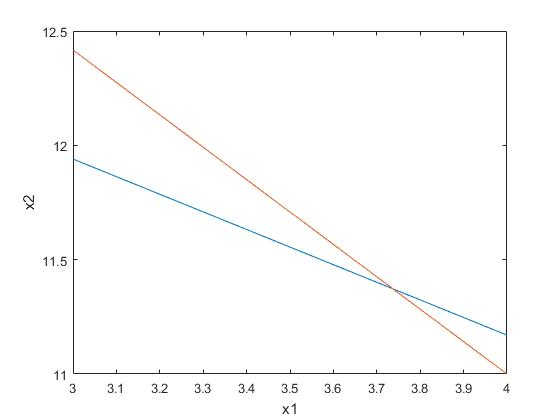
\includegraphics[width=\linewidth]{HW6-LineIntersect.jpg}
With $x_{1}$ on the x-axis, and $x_{2}$ on the y-axis we see $(x_{1},x_{2}) \approx (3.71,11.4)$
Back substituting these answers gives
\begin{align*}
f_{1}(x_{1},x_{2}) &= 0.77(3.71) + (11.4) = 2.8567 + 11.4 = \boxed{14.2567}
&	
\left| \Delta f_{1} \right| &= \left| 14.2567 -  14.25 \right| = 0.0067\\
f_{2}(x_{1},x_{2}) &= 1.2(3.71) + 1.7(11.4) = 4.4520 + 19.38 = \boxed{23.8320}
&
\left| \Delta f_{2} \right| &= \left| 23.8320 -  20 \right| = 3.8320
\end{align*}

I'm assuming the question is leading us to say that the system is ill positioned. While $f_{1}$ is roughly accurate, $f_{2}$ is much farther off than it could be.
\[
\begin{vmatrix}
0.77	&	1	\\
1.2		&	1.7
\end{vmatrix}
= (0.77)(1.7) - 1(1.2) = 1.3090 - 1.2 = \boxed{0.1090}
\]
Which is close to zero.

\setcounter{problem}{7}
\begin{problem}
Given the equations
\begin{align*}
2x_{1}	-6x_{2}	-x_{3}	&=	-38\\
-3x_{1}	-x_{2}	+7x_{3}	&=	-34\\
-8x_{1}	+x_{2}	-2x_{3}	&=	-20
\end{align*}
\begin{enumerate}[(a)]
\item Solve by Gauss elimintaion with partial pivoting. As part of the computation, use the diagonal elements to calculate the determinant. Show all steps of the computation.
\item Substitute your results into the original equations to check your answers.
\end{enumerate}
\end{problem}

\begin{align*}
&\left[ \begin{array}{ c c c : c }
2	&	-6	&	-1	&	-38	\\
-3	&	-1	&	7	&	-34	\\
-8	&	1	&	-2	&	-20
\end{array} \right]
&	
&\text{Pivot 1\&3}\longrightarrow
&
&\left[ \begin{array}{ c c c : c }
-8	&	1	&	-2	&	-20	\\
-3	&	-1	&	7	&	-34	\\
2	&	-6	&	-1	&	-38
\end{array} \right]
\\
&\left[ \begin{array}{ c c c : c }
-8	&	1	&	-2	&	-20	\\
-3	&	-1	&	7	&	-34	\\
2	&	-6	&	-1	&	-38
\end{array} \right]
&	
&\substack{(-0.375)\\(0.25)}\longrightarrow
&
&\left[ \begin{array}{ c c c : c }
-8	&	1			&	-2		&	-20		\\
0	&	-1-0.375	&	7+0.75	&	-34+7.5	\\
0	&	-6+0.25		&	-1-0.5	&	-38-5
\end{array} \right]
\\
&\left[ \begin{array}{ c c c : c }
-8	&	1		&	-2		&	-20		\\
0	&	-1.375	&	7.75	&	-26.5	\\
0	&	-5.75	&	-1.5	&	-43
\end{array} \right]
&	
&\text{Pivot 2\&3}\longrightarrow
&
&\left[ \begin{array}{ c c c : c }
-8	&	1		&	-2		&	-20		\\
0	&	-5.75	&	-1.5	&	-43		\\
0	&	-1.375	&	7.75	&	-26.5
\end{array} \right]
\\
&\left[ \begin{array}{ c c c : c }
-8	&	1		&	-2		&	-20		\\
0	&	-5.75	&	-1.5	&	-43		\\
0	&	-1.375	&	7.75	&	-26.5
\end{array} \right]
&	
&(0.2391)\longrightarrow
&
&\left[ \begin{array}{ c c c : c }
-8	&	1		&	-2			&	-20		\\
0	&	-5.75	&	-1.5		&	-43		\\
0	&	0		&	7.75+0.3587	&	-26.5+10.2826
\end{array} \right]
\\
&\left[ \begin{array}{ c c c : c }
-8	&	1		&	-2		&	-20		\\
0	&	-5.75	&	-1.5	&	-43		\\
0	&	0		&	8.1087	&	-16.2174
\end{array} \right]
\end{align*}
\begin{align*}
x_{3} &= \left(\frac{-16.2174}{8.1087}\right) = -2\\
x_{2} &= \left(\frac{-43-1.5(2)}{-5.75}\right) = 8\\
x_{1} &= \left(\frac{-20-2(2)-8}{-8}\right) = 4
\end{align*}

\begin{align*}
2x_{1}	-6x_{2}	-x_{3}	&=	& 2(4)		-6(8)	+2		&= -38 \\
-3x_{1}	-x_{2}	+7x_{3}	&=	& -3(4)	-8		-7(2)	&= -34\\
-8x_{1}	+x_{2}	-2x_{3}	&=	& -8(4)	+8		+2(2)	&= -20
\end{align*}

And surprisingly, even with floating point arithmetic, the solutions are exact.

\end{document}